\documentclass[12pt]{article}

% Packages
\usepackage{amsmath}
\usepackage[margin = 0.75 in]{geometry}
\usepackage[shortlabels]{enumitem}
\usepackage{tikz}

% Configuration
\title{15.2.9. (pg. 1059)}
\author{Arnav Patri}
\pagestyle{empty}

% Notation Macros
\renewcommand{\d}{\text{d}}

\begin{document}
	\maketitle
	\thispagestyle{empty}
		\[f(x, y) = xy\]
		\[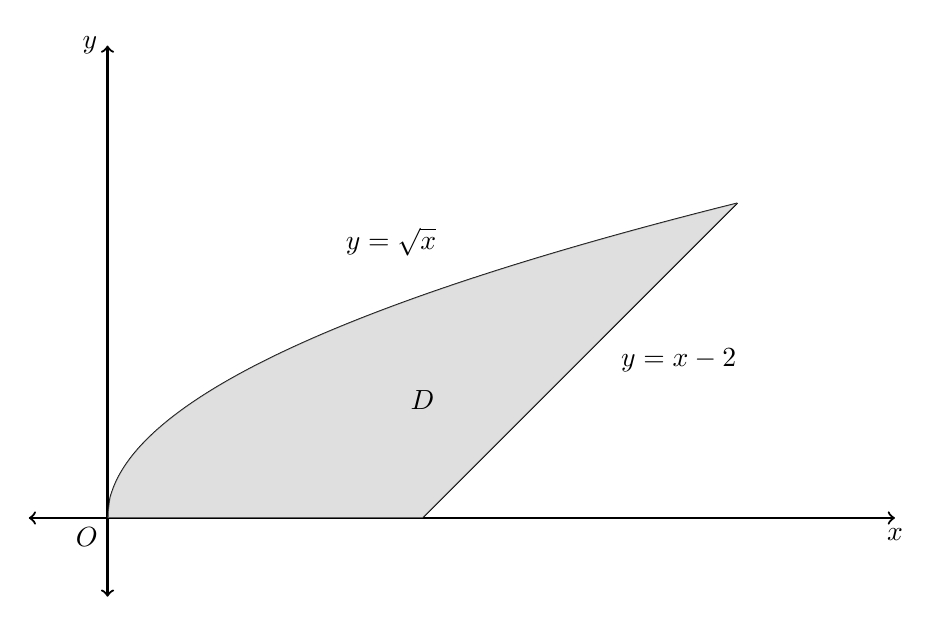
\begin{tikzpicture}[scale = 2]
			\draw[<->, thick] (-0.5, 0) -- (5, 0) node[below]{$x$};
			\draw[<->, thick] (0, -0.5) -- (0, 3) node[left]{$y$};
			\node[anchor = north east] at (0, 0) {$O$};
			\draw[domain = 0:4, smooth, samples = 300, variable = \x] plot({\x}, {sqrt(\x)});
				\node[above] at (1.8, 1.6) {$y = \sqrt{x}$};
			\draw[] (2, 0) -- (4, 2);
				\node[right] at (3.2, 1) {$y = x - 2$};
			\fill[lightgray, opacity = 0.5, domain = 0:4, smooth, samples = 300, variable = \x] (0, 0) -- plot({\x}, {sqrt(\x)}) -- (2, 0);
			\node at (2, 0.75) {$D$};
		\end{tikzpicture}\]
	\begin{enumerate}[(a)]
		\item 
			Express the double integral $\iint\limits_D f(x, y)\,\d A$ as an iterated integral for the given function $f$ and region $D$. 
			\begin{align*}
				y &= \sqrt{x} &
						y &= x - 2 \\
				x &= y^2 &
						x &= y + 2
			\end{align*}
			\begin{align*}
				y^2 &= y + 2 \\
				0 &= y^2 - y - 2 \\
					&= (y - 2)(y + 1) \\
				y &= -1, 2	
			\end{align*}
			\[\iint\limits_D f(x, y)\,\d A = \int_0^2\int_{y^2}^{y + 2} xy\,\d x\,\d y\]
		\item
			Evaluate the iterated integral.
			\begin{align*}
				\int_0^2\int_{y^2}^{y + 2} xy\,\d x\,\d y &= \int_0^2\left[\frac{x^2y}{2}\right]_{y^2}^{y + 2}\d y \\
					&= \int_0^2\left[\frac{(y + 2)^2y}{2} - \left(\frac{y^5}{2}\right)\right]\d y \\
					&= \int_0^2\left[\frac{y^3 + 4y^2 + 4y - y^5}{2}\right]\d y \\
					&= \left[-\frac{y^6}{12} + \frac{y^4}{8} + \frac{2y^3}{3} + y^2\right]_0^2 \\
					&= -\frac{64}{12} + \frac{16}{8} + \frac{16}{3} + 4 \\
					&= 6
			\end{align*}
		\begin{enumerate}[I]
			\item
				asdf
			\item
			\item
			\item	
		\end{enumerate}
	\end{enumerate}
\end{document}
